\documentclass[a4paper, 12pt]{article}
\usepackage[top=2cm, bottom=2cm, left=2.5cm, right=2.5cm]{geometry}
\usepackage[utf8]{inputenc}
\usepackage{amsmath, amsfonts, amssymb}
\usepackage{float}
\usepackage{graphicx}
\usepackage{caption}
\usepackage{subcaption}
\usepackage[brazil]{babel}
\usepackage{indentfirst}

\begin{document}

\section{Introdução}

\textbf{1. Histórico}

\textbf{2. Conceitos de Automação industrial}

\textbf{2.1. Automação e mão de obra}

\textbf{2.2. Automação e controle}

\textbf{2.3. Automação e eletrônica}

\textbf{3. Sistemas de Automação}

\textbf{4. Processos industriais}

\textbf{VANTAGENS DA AUTOMAÇÃO}

\subsection{Justificativa}

Enfatizar a Não parada da linha de produção

\subsection{Objetivo Geral}

Este trabalho tem o propósito de/pretende/visa/ mostrar a importância da 
ultilização de ferramentas de simulação para a programação de máquinas de
automação de processos industriais.

(citar a bancada Festo?)

\subsection{Objetivo Especifico}

\begin{itemize}
  \item Projetar uma linha de produção industrial
  \item Implementar o projeto utilizando CLP a Ladder Logic
  \item Simular a implementação usando o Factory I/O
  \item Utilizar a implementação na planta real (Bancada Festo?)
  \item Verificar ...
\end{itemize}

\section{Referencial Teórico}

	\subsection{Controlador Lógico Programável}
	
		O Controlador Lógico Programável - \textit{CLP} (do inglês, \textit{Programmable Logic Computer - PLC}),
		é uma ferramenta fundamental na industria, pois foi projetado para o uso em um
		ambiente industrial, capaz de resistir às adversidades presentes em uma fábrica,
		tais como água, temperaturas extremas, impactos, sujeira em excesso, dentre outras.
		
		A International Electrotechinical Commission - \textit{IEC}, na norma 61131, define
		o CLP como sendo um sistema eletrônico operando digitalmente, projetado 
		para uso em um ambiente industrial, que usa uma  	memória programável para armazenar
		internamente instruções orientadas para o usuário implementar funções especificas,
		tais como lógica, seqüencial, temporização, contagem e aritmética, para controlar,
		através de entradas e saídas	digitais ou analógicas, vários tipos de máquinas ou 
		processos.
	
		O CLP é amplamente utilizado para o controle de processos industriais, por apresentar
		alguns benefícios como a facilidade de instalação e programação, compatibilidade de rede,
		verificação de defeitos, confiabilidade, além de reduzir muito a quantidade de fios e cabos
		presente nos circuitos de controle a relé, como mostram as Figuras \ref{fig:clp-control-panel} e \ref{fig:rele-control-panel}.
		
		\begin{figure}[H]
			\centering
			\begin{minipage}{.5\textwidth}
			  \centering
			  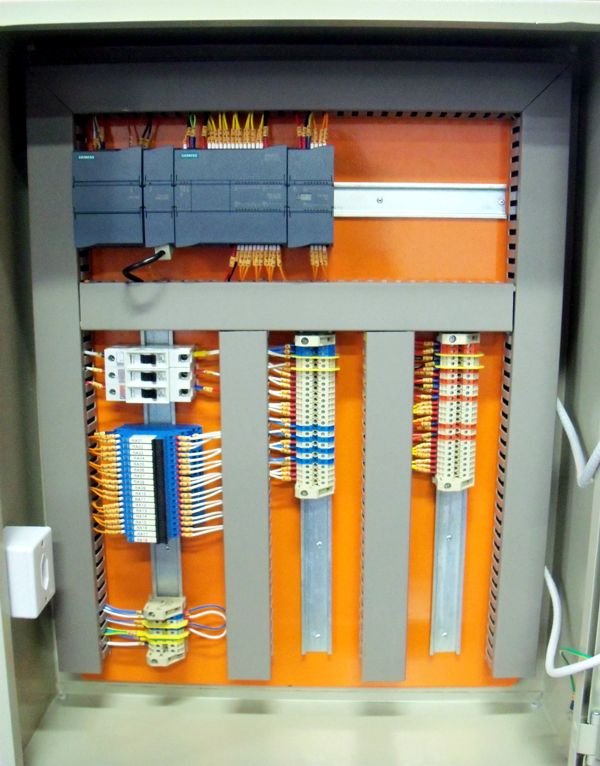
\includegraphics[width=.65\linewidth]{figures/CLPControlPanel.png}
			  \captionof{figure}{Painel de controle com CLP}
			  \label{fig:clp-control-panel}
			\end{minipage}% não tirar o %
			\begin{minipage}{.5\textwidth}
			  \centering
			  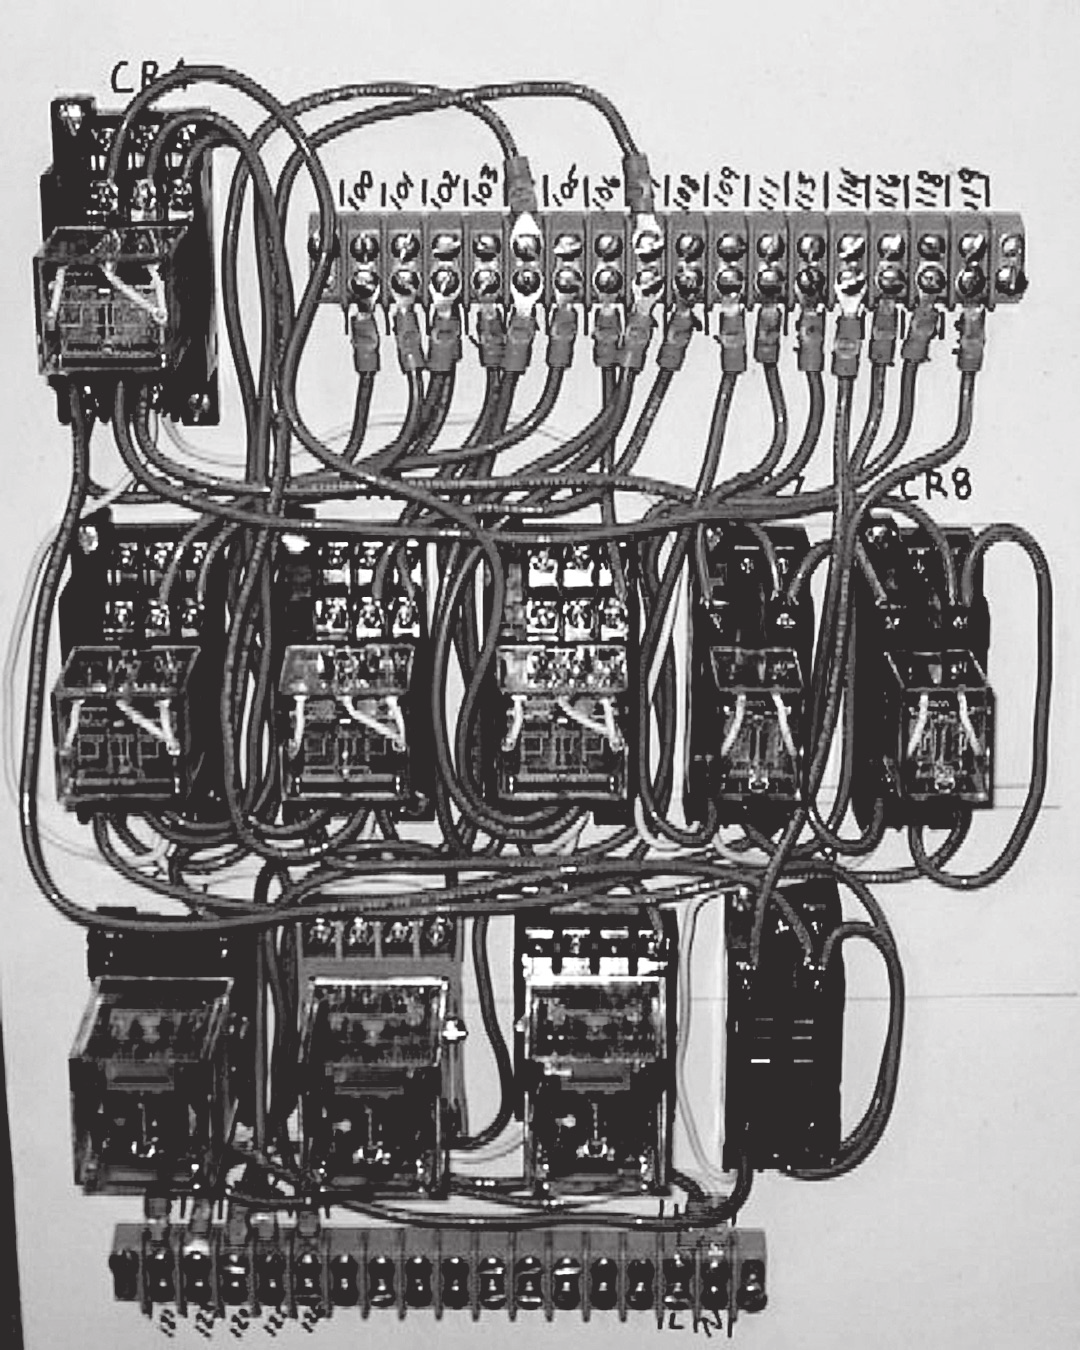
\includegraphics[width=.65\linewidth]{figures/ReleControlPanel.png}
			  \captionof{figure}{Painel de controle a relés}
			  \label{fig:rele-control-panel}
			\end{minipage}
		\end{figure}
	
		Os CLPs tem algumas outras vantagens em relação aos controles a relé convencionais. Enquanto os relés
		precisam ser instalados para executar uma função específica, e quando o sistema precisa de uma modificação,
		os condutores do relé precisam ser substituídos ou modificados, os CLPs são mais flexíveis ao permitir
		que o usuário apenas crie ou altere a lógica do programa armazenado nele.
		Em controles a relé, o modo como os relés são interconectados regem as relações entre	entradas e saídas,
		em um CLP, o usuário do programa é quem determina estas relações. A Figura \ref{fig:clp-io-relation} mostra as relações:
	
		\begin{figure}[H]
			\centering
			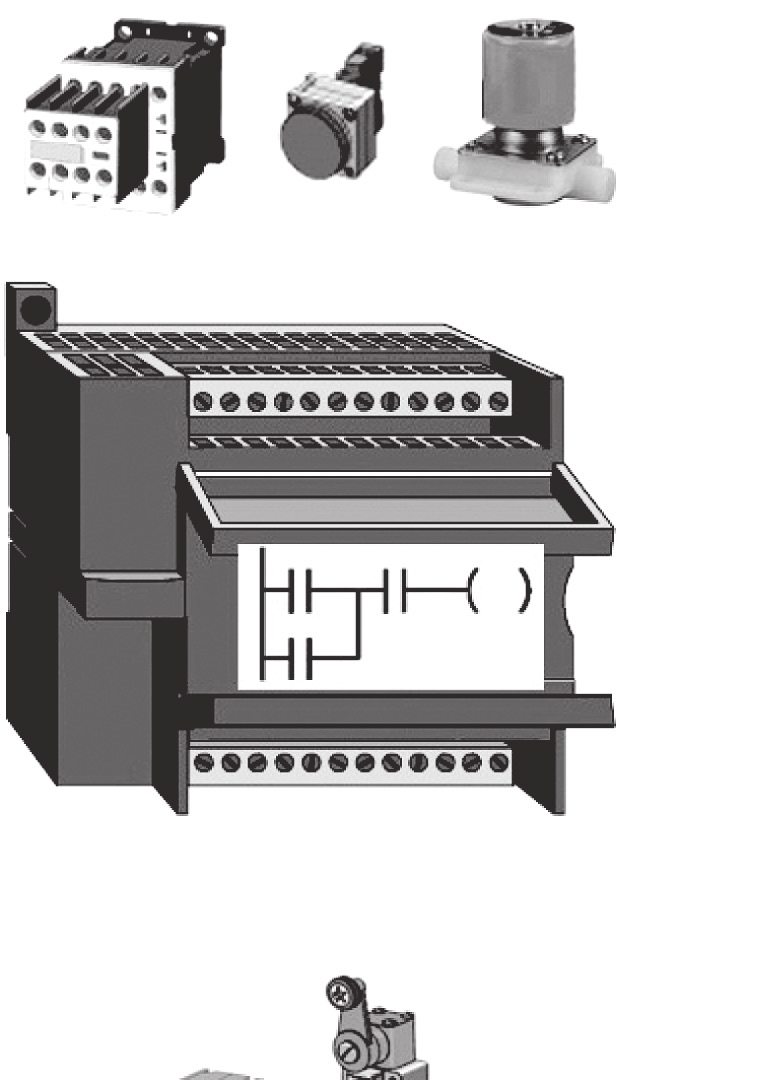
\includegraphics[scale=0.5]{figures/CLPInputOutputRelation.png}
			\caption{Entradas e Saídas de um CLP}
			\label{fig:clp-io-relation}
		\end{figure}
	
		Os CLPs tem grande capacidade de comunicação. Um CLP pode comunicar-se com outros CLPs ou qualquer outro
		equipamento do computador criando uma rede capaz de realizar funções como supervisão do controle, coleta de dados,
		dispositivos de monitoramento, e permitindo também baixar e transferir programas.
	
		\subsubsection{Siemens SIMATIC S7-1200}
		
			O S7-1200 é um controlador fabricado pelo conglomerado industrial alemão Siemens. Ele oferece flexibilidade e poder
			para controlar uma variedade de dispositivos em ambientes industriais. Tem uma estrutura compacta, medindo 11 x 10 x 7,5 centimetros,
			uma configuração flexível, e um poderoso conjunto de instruções para controlar uma ampla variedade de aplicações.
		
			Podemos ver algumas partes do S7-1200 na Figura \ref{fig:s7-1200-parts}:
			
			\begin{figure}[H]
				\centering
				\begin{minipage}{.5\textwidth}
			  		\centering
			  		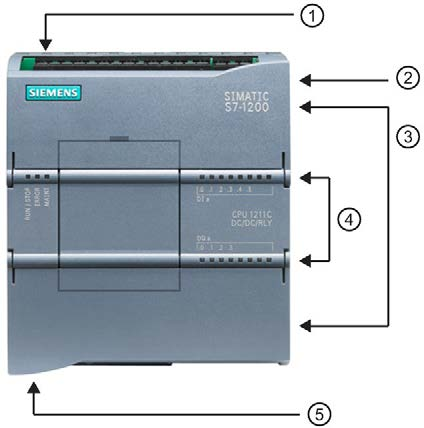
\includegraphics[width=.65\linewidth]{figures/s7-1200_parts.png}
				  \captionof{figure}{CLP Siemens S7-1200.}
				  \label{fig:s7-1200-parts}
				\end{minipage}% não tirar esse o %
				\begin{minipage}{.5\textwidth}
			  		\centering
			  		\begin{enumerate}
			  			\item Conector da fonte de alimentação
			  			\item Espaço para cartão de memória (atrás da tampa)
			  			\item Conectores de fios (atrás da tampa)
			  			\item LEDs de status para entradas e saídas
			  			\item Conector PROFINET (em baixo do CLP)
			  		\end{enumerate}
				\end{minipage}
			\end{figure}
		
			\textbf{TODO}
			1.2 Capacidade de expansão
		
			A.6 e A.6.3 (Pegar quantidade de portas e etc)

	\subsection{Linguagens de Programação de um CLP}
	
		Um CLP pode ser programado usando algumas diferentes linguagens de programação, (Definição de linaguem de programação???).
		
		Para fins de pradonização, o IEC na norma 61131-3 sobre Linguagens de Programação,
		definiu os padrões das linguagens utilizadas na programação de um CLP.

		Algumas linguagens usadas para programar um CLP (Petruzella, 2014):
		
		\begin{itemize}
			\item \textbf{Bloco de Funções (FBD)}
			
				Representação gráfica de fluxo de procedimentos que interconecta blocos simples
				e complexos.
				
			\item \textbf{Diagrama Ladder (LD)}
			
				Uma representação gráfica de processos com degraus lógicos semelhantes aos esquemas
				com lógica a relé.
				
			\item \textbf{Mapa de Funcção Sequencial (SFC)}
			
				Representação gráfica de passos, ações e transições interligadas.
				
			\item \textbf{Lista de Instruções (IL)}
			
				Linaguagem de baixo nível, baseada em texto e que usa instruções mnemônicas.
				
			\item \textbf{Texto Estruturado (ST)}
			
				Uma linguagem de alto nível, baseada em texto, como C, e que foi desenvolvida
				especificamente para aplicações de controle industrial.
				
		\end{itemize}
		
		A Figura \ref{fig:progam-language-clp} ilustra o padrão IEC 61131-3 de linguagens para a programação de CLP.

		\begin{figure}[H]
			\centering
			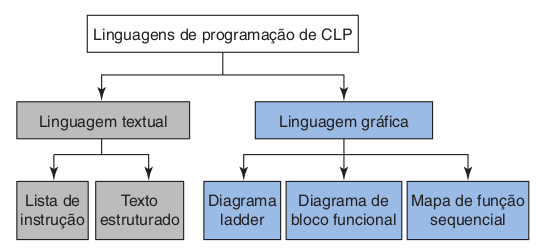
\includegraphics[scale=0.5]{figures/programming_language_for_CLP_IEC-61131-3.png}
			\caption{Linguagens de programação para CLP. IEC 61131-3.}
			\label{fig:progam-language-clp}
		\end{figure}
		
		\textbf{TODO}
		\textbf{MELHORAR O TEXTO DESSA SUBSEÇÃO}
		
		\subsubsection{Ladder Logic - LD}
		
			A linguagem em diagrama ladder(ou Ladder Logic) é a linguagem mais utilizada para CLP (Petruzella, 2014)
			e é projetada para imitar a lógica a relé.
		
			A LD, como também é conhecida, é uma representação gráfica de dispositivos físicos
			como sensores, botoeiras, bobinas, entre outros.
			
			Os elementos do programa são organizados em linha horizontais conhecidadas como
			degraus que simulam um circuito elétrico. As linhas ficam entrer duas linhas
			verticais conhecidas como trilhos.
			
			Contadores, somadores, bobinas, temporizadores, contatos, entre outras várias
			operações de dados são organizados nos degraus do diagrama.
			O gráfico ao final da programação fica semelhante a uma escada(do inglês \textit{ladder}), por isso o nome.
			
			A Figura \ref{fig:ladder_basic_example} a seguir mostra a organização de um programa feito em Ladder:
			
			\begin{figure}[H]
				\centering
				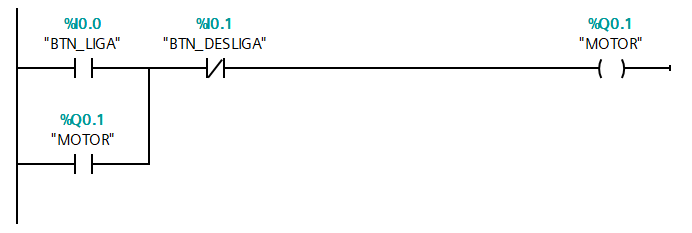
\includegraphics[scale=0.5]{figures/ladder_basic_example.png}
				\caption{Exemplo de um programa em Ladder.}
				\label{fig:ladder_basic_example}
			\end{figure}
			
			\textbf{TODO}
			\textbf{EXPLICAR RAPIDAMENTE O PROGRAMA}

	
	\subsection{TIA Portal v14}
	
		\textbf{TODO}
		DO manual:
		
		3. Software de programação
		
		3.2 pra pegar imagens
		
		6. Device configuration (Imagens tbm)
		
		7. Programming Concepts
		
		\subsubsection{Siemens S7-PLCSIM}
		
			\textbf{TODO}
	
	\subsection{Sistemas Supervisórios - SCADA}
		
		Os sistemas supervisórios exercem uma importante e essencial tarefa no contexto
		industrial: levar informações do processo industrial a quem está operando.
		O principal objetivo do sistema supervisório é ter uma visão do processo como um
		todo para permitir que o operador compreenda as etapas do processo e tome as ações
		necessárias para garantir o bom funcionamento do sistema.
		
		Com o sistema SCADA - \textit{Supervisory Control and Data Acquisition} é possível
		configurar a planta específica, realizar a aquisição dos dados e armazenar em um
		banco de dados, ou num planilha simples, dependendo da aplicação, além de fornecer
		informações do processo aos operadores.
		
		\begin{figure}[H]
			\centering
			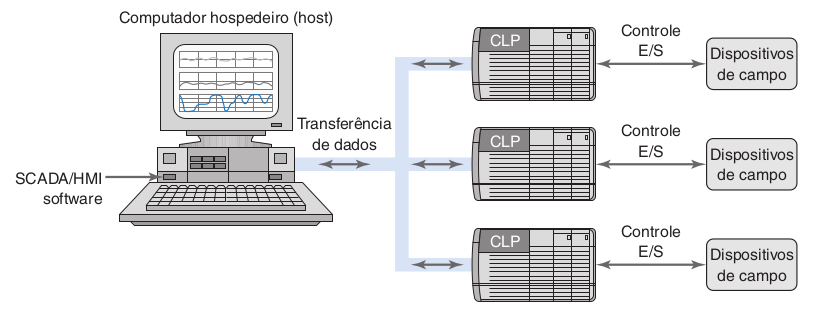
\includegraphics[scale=0.5]{figures/SCADA.png}
			\caption{Sistema SCADA.}
			\label{fig:scada}
		\end{figure}
		
		O sistema SCADA permite o ajuste de processos com precisão para a eficiência máxima, e
		independentemente do desempenho das funções de controle dos CLPs sobre os dispositivos
		de campo enquanto são supervisionados por um de programa SCADA/HMI rodando em um computador
		hospedeiro(host), como mostra a Figura \ref{fig:scada} acima. Operadores de controle do processo monitoram
		a operação do CLP no host e, se necessário, enviam os comandos de controle para os CLPs.
		
		É importante frisar que mesmo os sistemas supervisórios sendo quase que autosuficientes, é sempre
		importante a presença de operadores experientes e conhecedores do processo que está sendo controlado,
		pois quando ocorrem erros, apesar dos sistemas mais modernos indicarem a origem do erro, 
		há a possibilidade de conflitos e erros de interpretação por parte do software.

	\subsection{Bancada Festo}
	
		\textbf{TODO}
	
	\subsection{Factory I/O}
	
		O Factory I/O é um software de simulação 3D para aprender tecnologias de automação.
		Ele permite construir rapidamente um ambiente virtual usando as peças industriais
		mais comuns encontradas. O Factory I/O chama as simulações de cena, e ele possui diversas cenas de 
		apliações industriais típicas prontas para uso.		
		
		\begin{figure}[H]
			\centering
			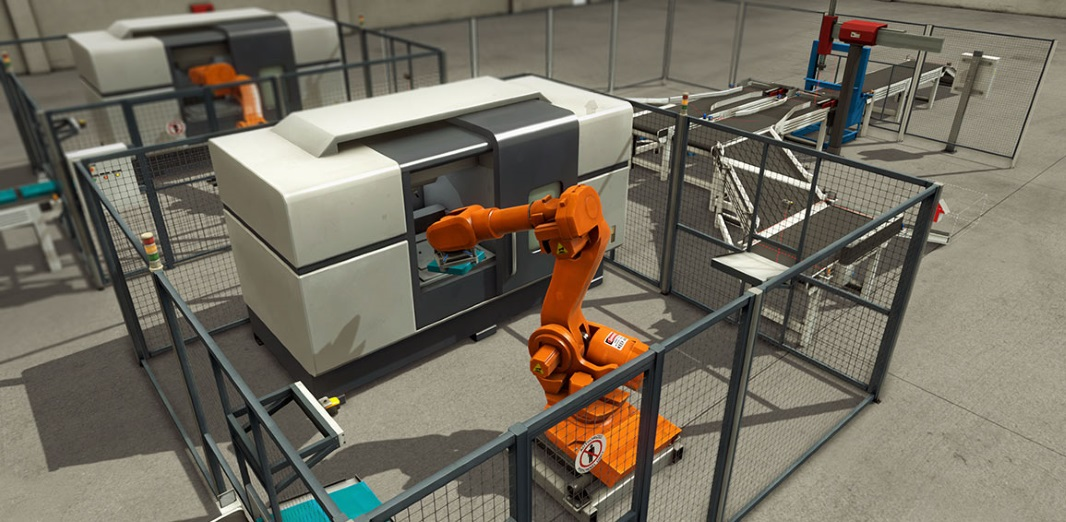
\includegraphics[scale=0.4]{figures/factory_io_1.jpg}
			\caption{Simualção no Factory I/O.}
			\label{fig:factory_simulation}
		\end{figure}
		
		O mais comum é utilizar o Factory I/O como plataforma de treinamento de CLP, pois
		os CLPs são os controladores mais comuns nas aplicações industriais. Porém, podem
		ser utilizados SoftPLC, microcontroladres, Modbus, entre várias outras tecnologias.
	
	\subsection{Digital Twin}
	
		\textbf{TODO}

\section{Metodologia da pesquisa}
	
	Nesta seção serão descritos os passos seguidos para o desenvolvimento do trabalho,
	as ferramentas e os métodos utilizados.
	A pesquisa foi dividida em 5 etapas:
	\begin{enumerate}
		\item Simular a planta real(bancada da Festo) no Factory I/O.
		\item Controlar a planta simulada utilizando o S7-PLCSIM.
		\item Controlar a planta simulada utilizando o CLP S7-1200.
		\item Controlar a planta real com o CLP S7-1200.
		\item Utilizar o CLP S7-1200 para controlar as plantas real e simulada ao mesmo tempo.
	\end{enumerate}
	
	Para esta pesquisa foram utilizadas os seguintes materiais:
		
	\begin{itemize}
		\item Factory I/O - software para simulação da planta
		\item TIA Portal versão 14 - software responsável pela programação do CLP
		\item Siemens S7-1200 - o controlador real
		\item S7-PLCSIM - o simulador de CLP integrado ao TIA Portal
		\item Bancada da Festo
	\end{itemize}
	
	\subsection{Criando uma simulação no Factory I/O}
	
		Primeiramente precisamos criar uma cena cliando na opção \textbf{New} no menu lateral esquerdo, como mostrado na
		Figura \ref{fig:creating-scene-step1}:
	
		\begin{figure}[H]
			\centering
			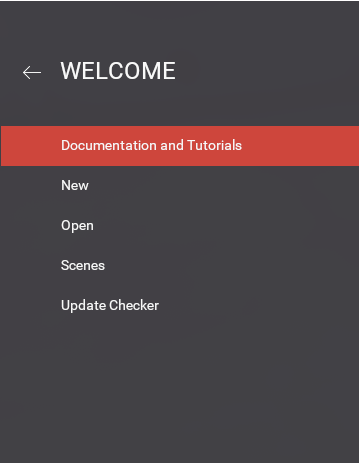
\includegraphics[scale=0.5]{figures/creating_scene_step_1.png}
			\caption{Criando uma nova cena no Factory I/O.}
			\label{fig:creating-scene-step1}
		\end{figure}
		
		Em seguida é necessário escolher quais equipamentos farão parte da cena. Na barra de ferramentas(\textbf{Toolbar}) há um botão
		de nome \textbf{Pallet window}, ao clicar sobre ele, uma barra lateral irá se expandir mostrando uma seleção de equipamentos
		industriais, basta escolher o que melhor se encaixa na simulação.
		
		\begin{figure}[H]
			\centering
			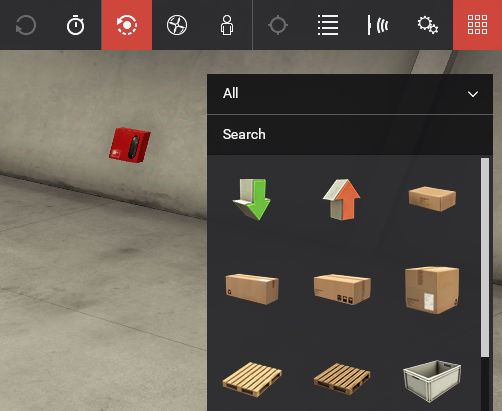
\includegraphics[scale=0.5]{figures/creating_scene_step_2.png}
			\caption{Equipamentos industriais disponiveis no Factory I/O.}
			\label{fig:creating-scene-step2}
		\end{figure}
		
		A Figura \ref{fig:creating-scene-step2} mostra o botão \textbf{Pallet window} destacado pelo retângulo amarelo.
		
		Agora basta escolher o equipamento procurando-o na lista de equipamentos. Opcionalmente pode-se filtrar os esquipamentos
		escrevendo seu nome na barra de pesquisa(\textbf{Search}) ou por categoria clicando na seção destacada pelo retângulo amarelo
		na Figura \ref{fig:creating-scene-step3}.
		
		\begin{figure}[H]
			\centering
			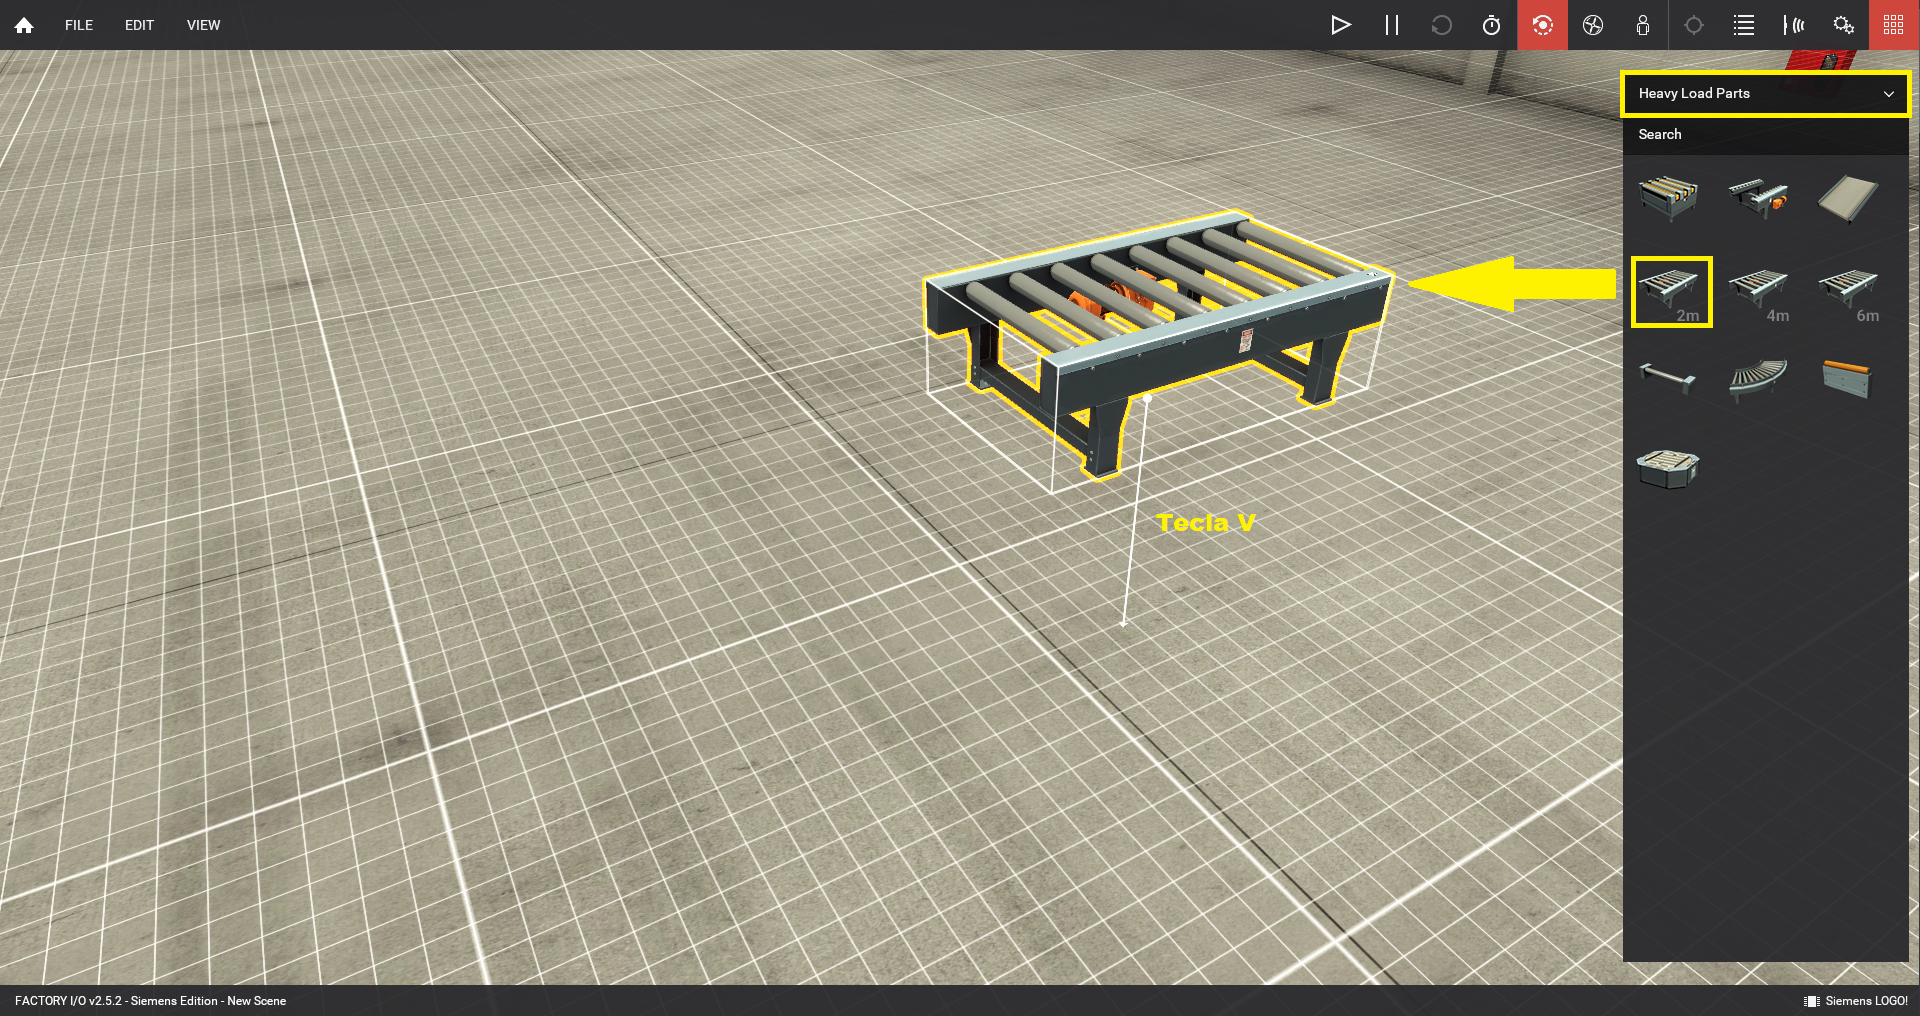
\includegraphics[scale=0.25]{figures/creating_scene_step_3.png}
			\caption{Filtrando e escolhendo o equipamento correto.}
			\label{fig:creating-scene-step3}
		\end{figure}		
		
		Para adicionar o equipamento à cena, basta clicar sobre ele e arrastar até o local desejado. Mantendo a \textit{tecla V}
		pressionada, podemos posicioná-lo no chão com mais facilidade. É possível ver estes passos na Figura \ref{fig:creating-scene-step3} acima.
		
		\textbf{TERMINAR}
	\subsection{Simulando a planta real no Factory I/O}

\section{Cronograma}

\section{Referencias Bibliográficas}

[1] Automação Industrial - Marco Antonio Ribeiro

[2] Controladores logicos programaveis - Frank D. Petruzella

[3] Automação Industrial na Prática - Frank Lamb

[4] Controladores Lógicos Programáveis - Claiton Moro Franchi

[5] A quarta revolução industrial - Klaus Schwab

[6] Automacao Industrial - Leandro Roggia \& Rodrigo Cardozo Fuentes

[7] Introdução à Automação - Mauro Spinola

[8] S7-1200 System Manual - Siemens

[9] IEC 61131

[10] IEC 61131-3

[11] https://docs.factoryio.com/ (acesso em 28/11/2022)

\end{document}
